% Harus dimuat terlebih dahulu, digunakan agar file PDF memiliki format karakter yang benar.
% Untuk informasi lebih lanjut, lihat https://ctan.org/pkg/cmap.
\RequirePackage{cmap}

% Format dokumen sebagai paper konferensi menggunakan aturan IEEEtran terbaru (v1.8b).
% Untuk informasi lebih lanjut, lihat http://www.michaelshell.org/tex/ieeetran/.
\documentclass[conference]{IEEEtran}[2015/08/26]

% Format encoding font dan input menjadi 8-bit UTF-8.
\usepackage[T1]{fontenc}
\usepackage[utf8]{inputenc}

% Format bahasa menjadi bahasa german dan inggris.
\usepackage[indonesian]{babel}

% Digunakan untuk tujuan demonstrasi.
\usepackage{mwe}

% Digunakan untuk menampilkan font dengan style yang lebih baik.
\usepackage[zerostyle=b,scaled=.75]{newtxtt}

% Digunakan untuk menampilkan tabel dengan style yang lebih baik.
\usepackage{booktabs}

% Digunakan untuk menampilkan gambar pada dokumen.
\usepackage{graphicx}

% Digunakan untuk menampilkan potongan kode.
\usepackage{listings}
\lstset{
  basicstyle=\ttfamily,
  columns=fixed,
  basewidth=.5em,
  xleftmargin=0.5cm,
  captionpos=b
}

% Digunakan agar backticks (`) dapat dirender pada PDF.
% Untuk informasi lebih lanjut, lihat https://tex.stackexchange.com/a/341057/9075.
\usepackage{upquote}

% Digunakan untuk menyeimbangkan bagian akhir dokumen dengan dua kolom.
\usepackage{balance}

% Digunakan untuk menampilkan pustaka.
\usepackage[square,comma,numbers,sort&compress]{natbib}

% Mengubah format ukuran teks pada natbib.
\renewcommand{\bibfont}{\normalfont\footnotesize}

% Menambah nama penulis ketika menggunakan perintah \citet.
% Untuk informasi lebih lanjut, lihat https://tex.stackexchange.com/a/76075/9075.
\usepackage{etoolbox}
\makeatletter
\patchcmd{\NAT@test}{\else \NAT@nm}{\else \NAT@hyper@{\NAT@nm}}{}{}
\makeatother

% Digunakan untuk menambah hyperlink pada referensi.
\usepackage{hyperref}

% Menonaktifkan warna dan bookmark pada hyperref.
\hypersetup{hidelinks,
  colorlinks=true,
  allcolors=black,
  pdfstartview=Fit,
  breaklinks=true
}

% Digunakan untuk membenarkan hyperref pada gambar.
\usepackage[all]{hypcap}

% Digunakan untuk menampilkan beberapa gambar
\usepackage[caption=false,font=footnotesize]{subfig}

\usepackage{stfloats}

% Tambahkan format tanda hubung yang benar di sini
\hyphenation{
  ro-ket
  me-ngem-bang-kan
  per-hi-tu-ngan
}

\begin{document}

  % Ubah kalimat berikut sesuai dengan judul penelitian.
\title{Kalkulasi Energi pada Roket Luar Angkasa \\ Berbasis \emph{Anti-Gravitasi}}

% Ubah kalimat-kalimat berikut sesuai dengan nama, institusi, alamat dan kontak penulis.
\author{
  \IEEEauthorblockN{Elon Reeve Musk}
  \IEEEauthorblockA{Departemen Teknik Dirgantara\\
    Fakultas Teknologi Dirgantara\\
    Institut Teknologi Sepuluh Nopember\\
    Surabaya, Indonesia 60111\\
    elon.musk@mhs.its.ac.id}

  \and
  \IEEEauthorblockN{Nikola Tesla}
  \IEEEauthorblockA{Departemen Teknik Dirgantara\\
    Fakultas Teknologi Dirgantara\\
    Institut Teknologi Sepuluh Nopember\\
    Surabaya, Indonesia 60111\\
    \url{https://nikolatesla.me}}

  \and
  \IEEEauthorblockN{Wernher von Braun}
  \IEEEauthorblockA{Departemen Teknik Dirgantara\\
    Fakultas Teknologi Dirgantara\\
    Institut Teknologi Sepuluh Nopember\\
    Surabaya, Indonesia 60111\\
    von.braun@td.its.ac.id}
}

% Digunakan untuk menampilkan judul dan deskripsi penulis.
\maketitle

  % Mengubah keterangan `Abstract` ke bahasa indonesia.
% Hapus bagian ini untuk mengembalikan ke format awal.
\renewcommand\abstractname{Abstrak}

\begin{abstract}

  % Ubah paragraf berikut sesuai dengan abstrak dari penelitian.
  Pada penelitian ini kami mengajukan \lipsum[1][1-12]

\end{abstract}

% Mengubah keterangan `Index terms` ke bahasa indonesia.
% Hapus bagian ini untuk mengembalikan ke format awal.
\renewcommand\IEEEkeywordsname{Kata kunci}

\begin{IEEEkeywords}

  % Ubah kata-kata berikut sesuai dengan kata kunci dari penelitian.
  Roket, Anti-gravitasi, Energi, Angkasa.

\end{IEEEkeywords}


  % Ubah bagian berikut sesuai dengan konten-konten yang akan dimasukkan pada dokumen
  \section{Pendahuluan}
\label{sec:pendahuluan}

Selama beberapa tahun terakhir, robot telah mengalami perkembangan yang signifikan dari robot beroda untuk edukasi \citep{goncalves2009} hingga robot manipulator untuk skala industri \citep{Blatnicky2020}.
Salah satu bentuk perkembangan lain dari robot tersebut adalah \emph{socially assistive robots} (SARs).
SARs merupakan jenis robot dalam bidang \emph{socially assistive robotics} yang menggabungkan aspek yang ada pada \emph{assistive robotics} dan \emph{socially interactive robotics} sehingga menjadikan SARs sebagai robot yang mampu memberikan bantuan kepada pengguna dalam bentuk interaksi sosial \citep{seifer2005}.

Namun, karena sifat dari SARs yang melibatkan interaksi langsung dengan pengguna, maka pengujian dari robot akan menjadi sulit dan beresiko bagi pengguna yang ikut terlibat dalam pengujian tersebut \citep{erickson2020}.
Salah satu solusi untuk mengatasi masalah tersebut adalah dengan melakukan pengujian secara virtual melalui simulasi robot.
Selain bisa meminimalisir resiko, penggunaan simulasi robot sebagai media pengujian robot juga bisa mengurangi biaya yang dibutuhkan dan menghemat waktu pengujian selama pengembangan robot tersebut \citep{takaya2016}.

Hingga saat ini sudah ada beberapa simulator yang bisa digunakan untuk menjalankan simulasi robot seperti Webots \citep{michel2004}, Gazebo \citep{koenig2004}, V-REP \citep{rohmer2013}, OpenAI Gym \citep{brockman2016}, dan lain sebagainya.
Namun, simulator-simulator tersebut hanyalah platform yang secara umum digunakan untuk membantu pengembangan robot melalui simulasi virtual.
Sedangkan pengembangan dari lingkungan simulasi dan kontroler robot untuk simulasi tersebut harus dibuat sendiri oleh pengembang robot.

Untuk itu, pada penelitian ini kami mengajukan penelitian terkait pengembangan lingkungan simulasi untuk pengujian SARs menggunakan ROS 2 dan Gazebo.
ROS 2 dan Gazebo sendiri dipilih karena tersedianya banyak library yang dapat membantu pengembangan maupun pengujian robot, terutama untuk simulasi.
Selain itu, dengan adanya ROS 2, kontroler robot yang diuji melalui simulasi bisa dengan mudah dipindahkan ke robot fisik untuk diuji secara langsung pada pengguna \citep{takaya2016}.

  \section{Penelitian Terkait}
\label{sec:penelitianterkait}

Beberapa penelitian sebelumnya telah berhasil dalam mengembangkan lingkungan simulasi untuk robot menggunakan ROS (Pendahulu ROS 2) dan Gazebo.
Seperti yang dilakukan Qian et al. \citep{qian2014} yang mengembangkan simulasi untuk robot \emph{manipulator}, Zhang et al. \citep{zhang2015} yang mengembangkan simulasi untuk robot \emph{quadrotor UAV}, dan Takaya et al. \citep{takaya2016} yang mengembangkan lingkungan simulasi untuk pengujian terhadap \emph{mobile robot}.
Namun, berbeda dengan penelitian yang telah dilakukan sebelumnya, penelitian yang akan kami lakukan memilih menggunakan ROS 2 agar kontroler robot yang dibuat untuk simulasi memiliki performa yang lebih baik serta dapat bekerja secara \emph{real-time} \citep{maruyama2016}.

Selain itu, penelitian lain juga telah dilakukan oleh Erickson et al. \citep{erickson2020} yang mengembangkan Assistive Gym, sebuah \emph{framework} simulasi untuk \emph{assistive robotics} berbasis OpenAI Gym.
\emph{Framework} simulasi tersebut kemudian digunakan oleh Clegg et al. \citep{clegg2020} untuk mengembangkan metode \emph{learning} melalui simulasi pada kolaborasi antara robot dengan manusia dalam membantu pemakaian baju pada manusia.
Namun, karena tidak menggunakan ROS, kontroler robot yang dibuat untuk simulasi yang menggunakan \emph{framework} tersebut perlu dibuat ulang ketika akan diujikan secara langsung pada pengguna menggunakan robot fisik.
Walaupun begitu, penelitian yang dilakukan oleh Zamora et al. \citep{zamora2016} menunjukkan bahwa simulasi yang ada pada OpenAI Gym juga bisa diintegrasikan pada ROS dan Gazebo, sehingga tidak menutup kemungkinan bahwa Assistive Gym juga bisa digunakan bersamaan dengan ROS 2 dan Gazebo.

  % Ubah judul dan label berikut sesuai dengan yang diinginkan.
\section{Desain dan Implementasi Sistem}
\label{sec:desainimplementasi}

% Ubah paragraf-paragraf pada bagian ini sesuai dengan yang diinginkan.

Pada cetak biru yang tertera pada Gambar \ref{fig:cetakbiru}. \lipsum[8]

% Contoh input gambar pada kolom.
\begin{figure} [ht]
  \centering
  % Ubah sesuai dengan nama file gambar dan ukuran yang akan digunakan.
  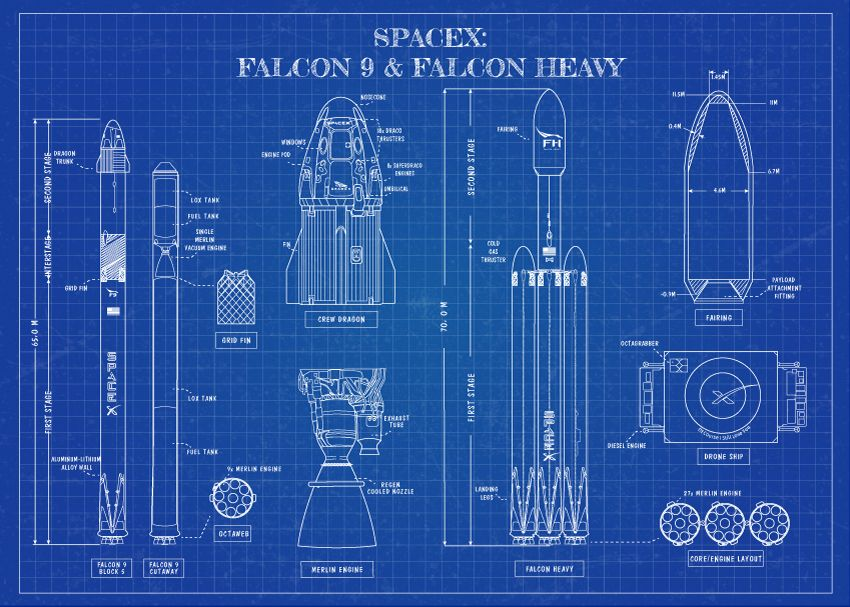
\includegraphics[width=0.4\textwidth]{gambar/cetakbiru.jpg}

  % Ubah sesuai dengan keterangan gambar yang diinginkan.
  \caption{Cetak biru roket yang akan diuji coba. \cite{cetakbiruspacex}}
  \label{fig:cetakbiru}
\end{figure}

\lipsum[9-11]

% Contoh pembuatan tabel.
\begin{table}
  \caption{Contoh tabel sederhana}
  \label{tab:tabelsederhana}
  \centering
  \begin{tabular}{lll}
    \toprule
    Heading1 & Heading2 & Heading3  \\
    \midrule
    One      & Two      & Three     \\
    Four     & Five     & Six       \\
    \bottomrule
  \end{tabular}
\end{table}

% Contoh pembuatan potongan kode.
\begin{lstlisting}[
  language=C++,
  caption={Program halo dunia.},
  label={lst:halodunia}
]
#include <iostream>

int main() {
    std::cout << "Halo Dunia!";
    return 0;
}
\end{lstlisting}

\lipsum[12]

% Contoh pembuatan daftar.
\begin{enumerate}
  \item \lipsum[13][1-4]
  \item \lipsum[13][5-8]
  \item \lipsum[13][9-12]
\end{enumerate}

\lipsum[14-15]

  % Ubah judul dan label berikut sesuai dengan yang diinginkan.
\section{Lorem ipsum}
\label{sec:loremipsum}

% Ubah paragraf-paragraf pada bagian ini sesuai dengan yang diinginkan.

% Contoh input beberapa gambar pada halaman.
\begin{figure*}
  \centering
  \subfloat[Hasil A]{\includegraphics[width=.4\textwidth]{example-image-a}
    \label{fig:hasila}}
  \hfil
  \subfloat[Hasil B]{\includegraphics[width=.4\textwidth]{example-image-b}
    \label{fig:hasilb}}
  \caption{Contoh input beberapa gambar.}
  \label{fig:hasil}
\end{figure*}

\lipsum[16-18]

% Contoh input potongan kode dari file.
\lstinputlisting[
  language=Python,
  caption={Program perhitungan bilangan prima.},
  label={lst:bilanganprima}
]{program/bilangan-prima.py}

\lipsum[19-20]

  % Ubah judul dan label berikut sesuai dengan yang diinginkan.
\section{Kesimpulan}
\label{sec:kesimpulan}

% Ubah paragraf-paragraf pada bagian ini sesuai dengan yang diinginkan.

\lipsum[21-23]


  % Menampilkan daftar pustaka dengan format IEEE
  \bibliographystyle{IEEEtranN}
  \bibliography{pustaka/pustaka.bib}

  % Menyeimbangkan bagian akhir di kedua kolom
  \balance

\end{document}
